%!TEX root = ../template.tex
%%%%%%%%%%%%%%%%%%%%%%%%%%%%%%%%%%%%%%%%%%%%%%%%%%%%%%%%%%%%%%%%%%%%
%% chapter6.tex
%% NOVA thesis document file
%%
%%%%%%%%%%%%%%%%%%%%%%%%%%%%%%%%%%%%%%%%%%%%%%%%%%%%%%%%%%%%%%%%%%%%

\typeout{NT FILE chapter6.tex}%

\chapter{Software Testing}
\label{cha:test}


\epigraph{ \textit{This chapter documents the software testing done throughout the development of the thesis. It highlights how the specific tests where done, in what context and their results.}}

Software testing was conducted specifically for the configuration of the code generation part of \gls{RAMSES}. This means that the goal was to ensure that the newly developed configuration options did not modify the runtime results of the generated software, hence maintaining the core goal of the input model.

\section{Feature Testing}
\label{sec:test_feature}

This type of testing is recurrent along the development, it serves to ensure that the features implemented are functioning as intended and that the previous version of the software has retained its functionality when new features were added.

\subsection{Feature Testing: August}
\label{sec:test_feature_one}

After the development of the first batch of features, the testing served to ensure that the previous version of the code generator was still working as intended and to validate the integration of the code generator configurator in the pipeline.

The report for the first volley of tests can be found in the Annex~\ref{label}, where it is explained the purpose of each individual test and the results they withheld.

The regression tests applied at this time were limited since the previous version of the software did not include any code generation customization, only the simple transition from model to code (\gls{M2T}), which, after generating a \gls{ROS} project in both the previous code generator and the at the time current one (with the first batch of features implemented), it was possible to verify that both generators still produced the same practical output, essentially, the code produced by both generators yields the same functionality.

The integration test part was done much more in depth since the goal was to intertwine the different new features and find out if they worked in perfect harmony as expected. The tests present in Table~\ref{tab:int_tests_1} were conducted.

\bgroup
\rowcolors{1}{}{GhostWhite}
\begin{xltabular}{\textwidth}{X X X X X}
	\caption{Feature dependency table}
	\label{tab:int_tests_1}\\
	\toprule
	\rowcolor{Gainsboro}%
	Test Case ID & Feature & Description & Expected Outcome \\
	\midrule
	TC-INT-01 & \Gls{identifier} Management & Check that \gls{identifier} config is applied in code, traceability, and report. & Same naming convention is visible in all outputs. \\
	TC-INT-02 & Comments & Verify comment style and formatting are preserved in all files. & All comments retain exact style and placement. \\
	TC-INT-03 & Traceability & Ensure model elements map to the correct code location and report entry. & JSON and HTML show accurate paths and line numbers. \\
	TC-INT-04 & Report Generation & Ensure generation metrics are passed from Java generator to report. & Report displays correct counts and settings. \\
	TC-INT-05 & Code Quality \& Report Sync & Verify quality checker warnings appear in both XML and report. & Both outputs show the same warning details. \\
	TC-INT-07 & Cross-Feature Stability & Test large models with custom \glspl{identifier}, comments, and style violations. & All features work together without breaking. \\
\end{xltabular}

After conducting these tests, the following was concluded:

\begin{itemize}
	\item \textbf{TC-INT-01 – \Gls{identifier} Consistency:} Verified that the \gls{identifier} configuration set in the \texttt{config.generator} model is applied consistently in generated C++ code and reflected in the traceability file as well as in the report.
	
	\item \textbf{TC-INT-02 – Comments:} Generated code containing both single-line and multi-line comments, verified that:
	\begin{enumerate}
		\item Acceleo templates correctly output the comments.
		\item Java generator preserves formatting.
	\end{enumerate}
	
	\item \textbf{TC-INT-03 – Traceability Link Accuracy:} Confirmed that model elements are mapped to the correct files and line numbers in generated code, and that these mappings are:
	\begin{enumerate}
		\item Present in the \gls{JSON} traceability output.
		\item Referenced in the \gls{HTML} report.
	\end{enumerate}
	
	\item \textbf{TC-INT-04 – Report Generation Data Flow:} Metrics collected during generation (number of components, code quality warnings) are passed to the Acceleo generator rendered correctly in the report.
	
	\item \textbf{TC-INT-05 – Code Quality \& Report Synchronization:} Triggered a known style violation in the model, generated code, and verified that:
	\begin{enumerate}
		\item The code quality checker detects it and outputs XML accurately referencing it.
		\item The Java generator correctly embeds this warning into the final HTML reportx.
	\end{enumerate}
	
	\item \textbf{TC-INT-07 – Cross-Feature Stability:} Used a large, complex model with:
	\begin{itemize}
		\item Custom \glspl{identifier}
		\item Extensive comments
		\item Nested subcomponents
		\item Known style violations
	\end{itemize}
	Verified that all features (\gls{identifier} config, comments, traceability, reporting, quality checking) work together without breaking any module.
\end{itemize}


\section{Unit Testing}
\label{sec:test_unit}

In order to automate the testing of the added features as development progressed unit tests were developed. By comparing the functional version of the generated projects against a newly generated version of the same project, we are able to detect differences in the end result which can point out flaws when a branch of the code generation is modified. 

Essentially, what we test can be visually described by Figure~\ref{fig:testingFlowchart}.

\begin{figure}[htbp]
	\centering
	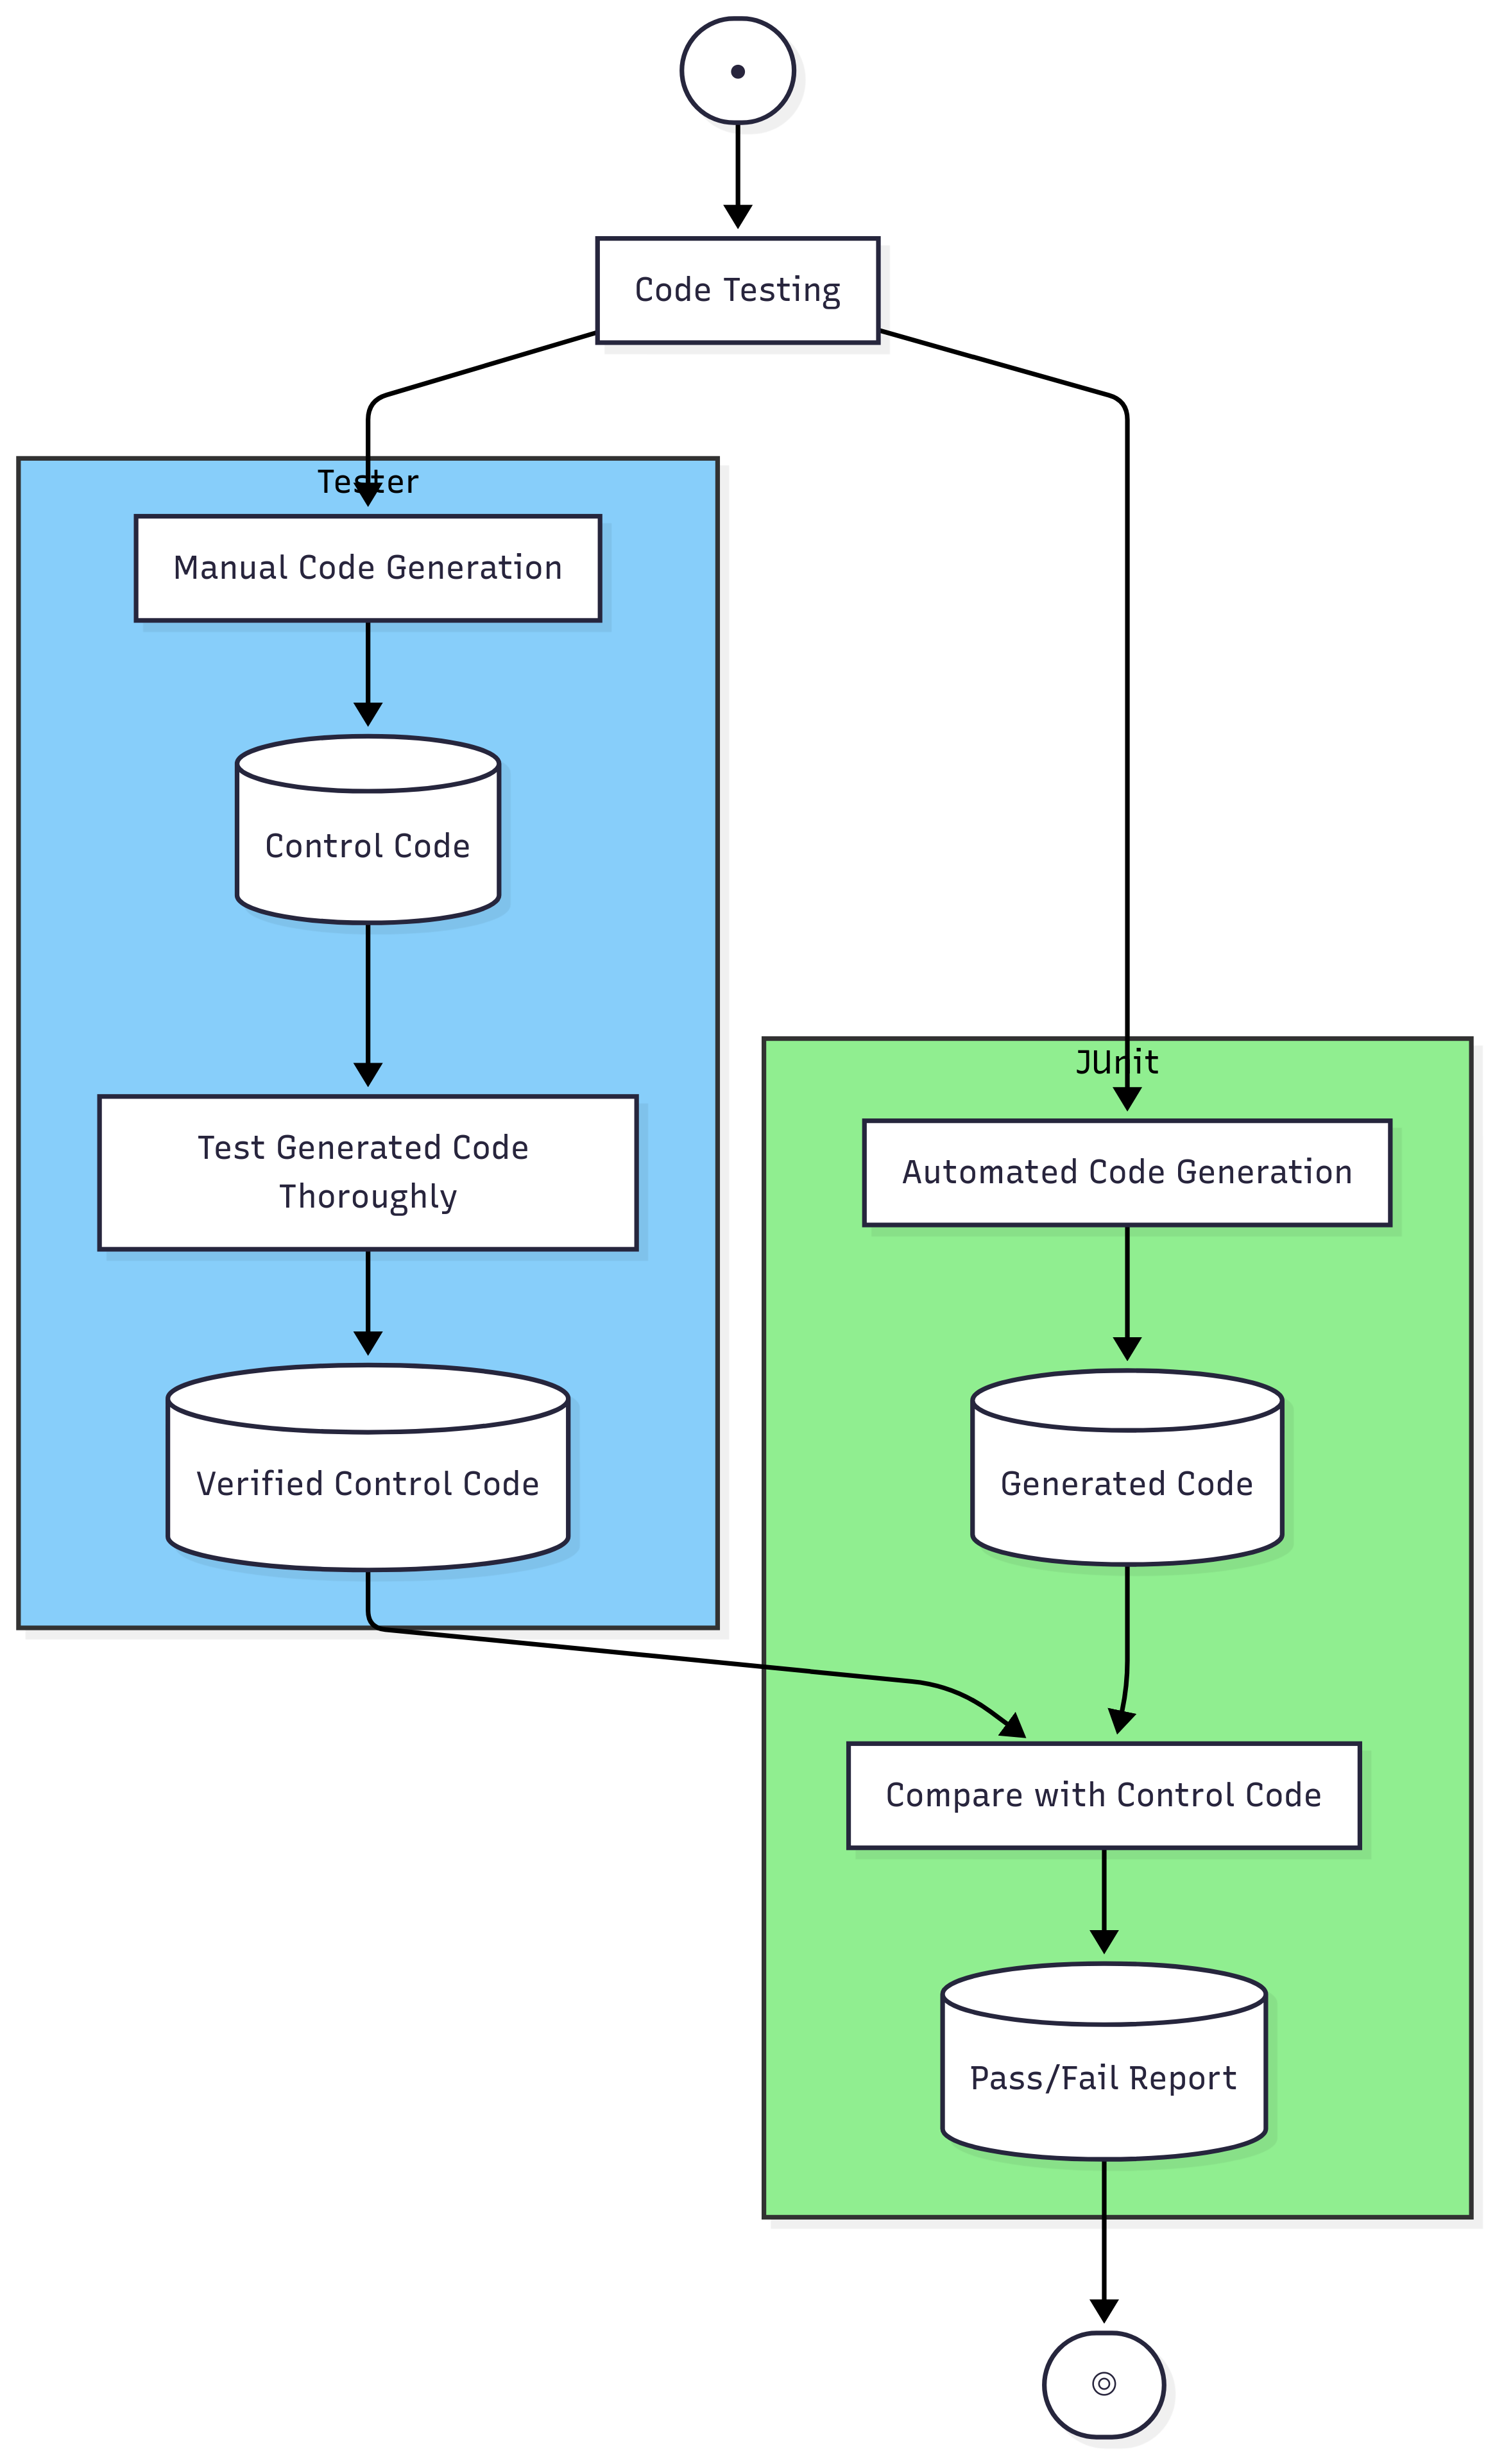
\includegraphics[width=0.55\textwidth]{testingFlowchart.png}
	\caption{Flowchart of the testing strategy for generated code (made by the author)}
	\label{fig:testingFlowchart}
\end{figure}

By using this architecture, it is only necessary to verify the correctness of the generated code once. The subsequent generations can be then compared to this already correct premise to determine errors or changes in the code that are not intended.

An obvious flaw of this model is that, not only does it need complete manual validation in the start, but it's also very rigid when it comes to file comparison, comparing each file line-by-line\footnote{The comparison is not overly rigid and allows for exceptions such as the generated date and order changes in \gls{XML} files.}.

These flaws can also be seen as benefits, since the code needs to be testes rigorously to ensure maximum code quality when generated. This can only be achieve by actually executing the generated projects and verifying their functionality.

The unit tests were made to be as flexible as possible, allowing for different configurations and different models to be tested in a single run, providing insights in multiple generated projects in a single test execution as can be observed in Figure~\ref{fig:testingResults1}.

\begin{figure}[htbp]
	\centering
	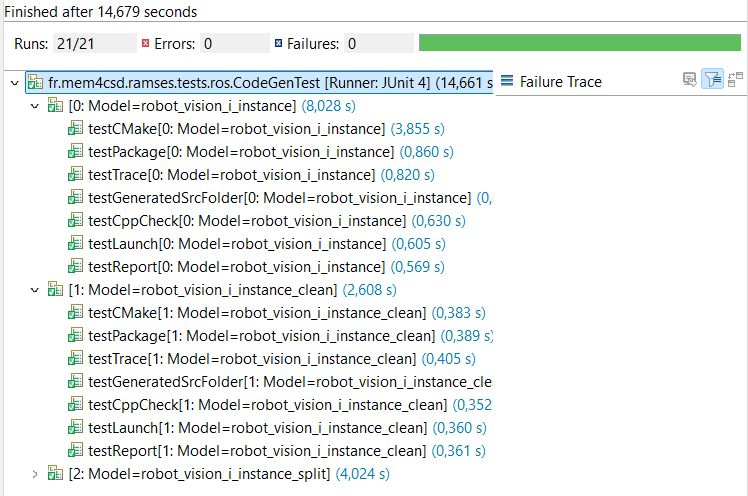
\includegraphics[width=0.55\textwidth]{testingResults1.png}
	\caption{Testing results of 3 different models}
	\label{fig:testingResults1}
\end{figure}

The tests also account for certain projects not generating certain files such as the traceability or the report file. This behavior is translated by simply skipping the test as can be observed in Figure~\ref{fig:testingResultsSkip1}. Similar tests also verify the existence of folders and files that are a requirement for any \gls{ROS} project and need to be present after generation.

\begin{figure}[htbp]
	\centering
	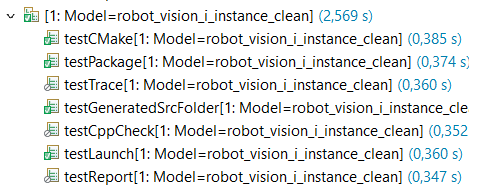
\includegraphics[width=0.55\textwidth]{testingResultsSkip1.png}
	\caption{Skipped Trace, CppCheck and Report files as those are not present}
	\label{fig:testingResultsSkip1}
\end{figure}

In addition, the test runs also validate the existence of executable both in the launch and make configurations, notably these executables have to exists in both files. 

As a guardrail, if files are present in the control project but not in the generated project that will generate an error and vice versa. This ensures that the generator produces only what is needed and no file is missing.

\bgroup
\rowcolors{1}{}{GhostWhite}
\begin{xltabular}{\textwidth}{X X X X X}
\caption{Feature dependency table}
\label{tab:reg_tests_1}\\
\toprule
\rowcolor{Gainsboro}%
Test Case ID & Feature & Description & Expected Outcome \\
\midrule
TC-REG-01 & Regression & Compare output with older version for unchanged models. & Output is functionally identical. \\
TC-REG-02 & Regression & Generate code for previously passing models. & Generation succeeds with no new errors. \\
TC-REG-03 & Regression & Measure generation time for unchanged models. & Timing does not exceed threshold. \\
TC-REG-04 & Regression & Test legacy models without new features enabled. & Output has no formatting or syntax changes. \\
\end{xltabular}




